% L'option handout permet de supprimer la barre de navigation
\documentclass[handout]{beamer}
\usepackage[utf8]{inputenc}
\usepackage[french]{babel}
\usepackage[T1]{fontenc}
\usepackage{amsmath}
% Pour pouvoir insérer des images
\usepackage{graphicx}
\usepackage{wrapfig}
\graphicspath{images/}
% Gestion des couleurs
\usepackage{color}
\definecolor{red}{RGB}{231, 76, 60}

\usepackage{minted}
\usemintedstyle{trac}

% Un joli thème flat
\usetheme{Rochester}

% Personnalisation du thème
\usecolortheme[named=red]{structure}
% Numéro de slides dans le footer
\setbeamertemplate{footline}[frame number]
\setbeamertemplate{blocks}[shadow=false]

\logo{
\includegraphics[width=1cm]{images/logoASI.jpg}}

\setbeamertemplate{footline}
{
	\leavevmode%
	\hbox{%
	\begin{beamercolorbox}[wd=.333333\paperwidth,ht=2.25ex,dp=1ex,center]{author in head/foot}%
		\usebeamerfont{author in head/foot}\insertsection
	\end{beamercolorbox}%
	\begin{beamercolorbox}[wd=.333333\paperwidth,ht=2.25ex,dp=1ex,center]{title in head/foot}%
		\usebeamerfont{title in head/foot}\insertsubsection
	\end{beamercolorbox}%
	\begin{beamercolorbox}[wd=.333333\paperwidth,ht=2.25ex,dp=1ex,right]{date in head/foot}%
		\usebeamerfont{date in head/foot}\insertshortdate{}\hspace*{2em}
		\insertframenumber{} / \inserttotalframenumber\hspace*{2ex}
	\end{beamercolorbox}}%
	\vskip0pt%
}

% ------------------------------------ %
% -- METADONNÉES DU DOCUMENT --------- %
\title{
	Bases de données aujourd'hui et bases de données NoSQL
}
\author{
	Antoine \textsc{Augusti}\\
	\vspace{5px}
	Thibaud \textsc{Dauce} \\
	\vspace{5px}
	Géraldine \textsc{Del Mondo} \\
}
\date{\today}

% Début du document
\begin{document}

	% Génération de la page de titre
	\begin{frame}[plain]
		\titlepage
	\end{frame}

	% Génération du sommaire
	\begin{frame}[plain]
		\frametitle{Sommaire}
		\tableofcontents
	\end{frame}

		% //////////////////////////////////////// %
% /// Architecture web et relationnel //// %
\section{Architecture web et relationnel}
	%% Architecture classique
	\subsection{Architecture classique}
	\begin{frame}
		\frametitle{Architecture classique}

		\begin{figure}[htb]
			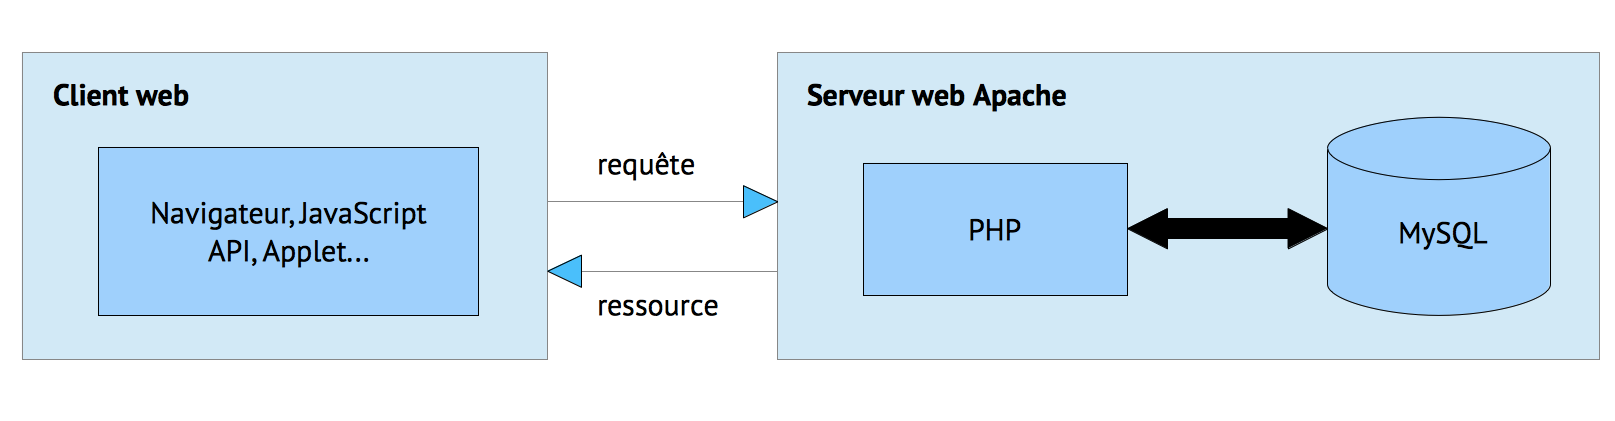
\includegraphics[width=1\textwidth]{images/LAMP.png}
		\end{figure}

		\begin{itemize}
			\item La plus commune : LAMP (Linux, Apache, MySQL, PHP) ;
			\item LEMP : Linux, Nginx, MySQL, PHP-FPM ;
			\item Stack JavaScript MEAN : MySQL (ou MongoDB), Express, AngularJS, Node.js.
		\end{itemize}

	\end{frame}

	%% Bilan architecture classique
	\subsection{Bilan architecture classique}
	\begin{frame}
		\frametitle{Bilan architecture classique}

		\textbf{Avantages :}
		\begin{itemize}
			\item Rapide à mettre en place (installation en un clic généralement) ;
			\item Optimisation possible, verticalement le plus souvent ;
		\end{itemize}

		\vspace{20px}

		\textbf{Inconvénients :}
		\begin{itemize}
			\item Il faut une expertise base de données.
		\end{itemize}

	\end{frame}

	%% Qu'est-ce qu'un ORM ?
	\subsection{Qu'est-ce qu'un ORM ?}
	\begin{frame}
		\frametitle{Qu'est-ce qu'un ORM ?}

		\begin{block}{Définition : ORM}
			L'\textbf{O}bject-\textbf{R}elationnal \textbf{M}apping est une technique qui simule une base de données orientée objet à partir d'une base de données relationnelle.
		\end{block}

		\vspace{2px}

		\begin{itemize}
			\item Fait la liaison entre le monde relationnel dans la couche stockage et le monde objet dans l'application ;
			\item Facilité de développement : \textit{pas besoin} d'une connaissance poussée du SQL ;
			\item Facilite les interactions avec la base de données pour les développeurs.
		\end{itemize}

		\vspace{2px}

		\begin{alertblock}{Les limites des ORM}
			Toujours \textbf{beaucoup} moins performant que des requêtes SQL optimisées.
		\end{alertblock}

	\end{frame}

	\begin{frame}
		\frametitle{ORM : exemple de requêtes}

		\begin{listing}[H]
			\inputminted[fontsize=\tiny, linenos=true]{php}{code/eloquent.php}
			\caption{Quelques requêtes basiques avec l'ORM Eloquent.}
		\end{listing}

	\end{frame}

		% //////////////////////////////////////// %
% /// Au delà du SQL : les BDs NoSQL ///// %
\section{Au delà du SQL : les BDs NoSQL}

	%% Pourquoi changer du relationnel ?
	\subsection{Pourquoi changer du relationnel ?}
	\begin{frame}
		\frametitle{Pourquoi changer du relationnel ?}

		Besoin d'une alternative vers les années 2004 avec l'arrivée du \textit{Big Data}.
		\begin{itemize}
			\item Des volumes de données important (plusieurs gigas, voire téraoctets) ;
			\item Un nombre de transactions très important, une forte demande de disponibilité et de temps de réponse ;
			\item Des bases de données réparties sur plusieurs centres de données ou continents ;
			\item Préférence pour l'ajout de petites machines plutôt qu'une configuration poussée des BDs.
		\end{itemize}

	\end{frame}

	%% Relâchement des contraintes de transactions
	\subsection{Relâchement des contraintes de transactions}
	\begin{frame}
		\frametitle{Relâchement des contraintes de transactions}

		Impossible de garantir les propriétés ACID des BDs relationnelles avec les nouvelles contraintes.\\
		\vspace{10px}
		De nouvelles propriétés \textbf{BASE} :
		\begin{itemize}
			\item \textit{Basic Availability} : système disponible dans son ensemble bien que certaines machines soient indisponibles ;
			\item \textit{Soft state} : l'état du système distribué peut changer, même sans nouvelles transactions ;
			\item \textit{Eventual Consistency} : En l'absence de nouvelles transactions, le système sera cohérent au bout d'un temps.
		\end{itemize}

	\end{frame}

	%% À quoi ressemble une BD NoSQL
	\subsection{À quoi ressemble une BD NoSQL}
	\begin{frame}
		\frametitle{À quoi ressemble une BD NoSQL}

		\begin{itemize}
			\item Un SGBD qui n'est pas structuré en tables et dont l'élément de base n'est pas un tuple mais dépend du type de BD NoSQL ;
			\item Un langage de requête non uniformisé, propre à chaque BD. Souvent au format JSON avec une API REST ;
			\item Une dénormalisation des données où certains enregistrements sont en partie ou entièrement dupliqués ;
			\item Type de base de données NoSQL à choisir en fonction de l'usage souhaité.
		\end{itemize}

	\end{frame}

		% ///////////////////////////////////////////// %
% /// Types de bases de données NoSQL ///// %
\section{Types de bases de données NoSQL}

	%% Bases de données clé-valeur
	\subsection{Bases de données clé-valeur}
	\begin{frame}
		\frametitle{Modélisation BD clé-valeur}

		\begin{itemize}
			\item \textbf{Modélisation :} la plus simple. À une clé, on associe une valeur. La valeur peut être de n'importe quel type (chaîne de caractères, entier, structure, objet sérialisé\dots).
		\end{itemize}

		\vspace{15px}
		Des exemples de paires clé-valeur avec des types différents.
		\vspace{5px}
		\begin{tabular}{|l|l|}
			\hline
			\textbf{Clé} & \textbf{Valeur} \\ \hline\hline
			pays.id-42 & \{"id":42,"name":"Chad"\} \\ \hline
			statistiques.nombre-visiteurs & 1337 \\ \hline
			configuration.periode-gratuite & false \\ \hline
			articles.categories-sport.latest & [22, 45, 67, 200, 87] \\ \hline
		\end{tabular}
	\end{frame}

	\begin{frame}
		\frametitle{BD clé-valeur en détail}
		\begin{itemize}
			\item \textbf{Opérations} : création d'une paire clé-valeur, suppression, accès à une valeur à l'aide de la clé, incrémentation et décrémentation d'une valeur ;
			\item On peut définir la durée de vie d'une paire clé-valeur ou adopter une politique \textit{least recently used} ;
			\item Stockage en RAM pour accélérer les temps de lecture. Mécanisme de reprise en cas de crash ;
			\item \textbf{Cas d'utilisation :} cache d'une autre BD, comptage d'éléments, gestion de files d'attente, opérations ensemblistes\dots
			\item \textbf{Principaux acteurs :} Redis, Memcached, Riak.
		\end{itemize}
	\end{frame}

	\begin{frame}
		\frametitle{Commandes sous Redis}

		\begin{listing}[H]
			\inputminted[fontsize=\tiny, linenos=true]{text}{code/commandesRedis.txt}
			\caption{Quelques commandes Redis en console.}
		\end{listing}
	\end{frame}

	%% Bases de données document
	\subsection{Bases de données orientées documents}
	\begin{frame}
		\frametitle{Bases de données orientées documents}

		\begin{itemize}
			\item \textbf{Modélisation :} aucun schéma fixe, un document peut contenir n'importe quel type d'information ;
			\item Optimisation horizontale ;
			\item \textbf{Opérations :} utilise le JSON pour les requêtes et l'améliore pour le stockage (BSON) ;
			\item Facile d'accès (API REST, shell\dots) ;
			\item \textbf{Cas d'utilisation :} base de données principalement utilisées pour du stockage ;
			\item \textbf{Principaux acteurs :} MongoDB, CouchDB, CouchBase.
		\end{itemize}
	\end{frame}

	\begin{frame}
		\frametitle{Exemple d'un document}

		\begin{listing}[H]
			\inputminted[fontsize=\tiny, linenos=true]{json}{code/exemple-document.json}
			\caption{Exemple d'un document JSON.}
		\end{listing}
	\end{frame}

	\begin{frame}
		\frametitle{Exemples de requêtes MongoDB}

		\begin{listing}[H]
			\inputminted{javascript}{code/requeteMongoFind.js}
			\caption{Exemple de requête find sur MongoDB.}
			\label{findMongoDB}
		\end{listing}
	\end{frame}

	\begin{frame}
		\frametitle{Exemples de requêtes MongoDB}

		\begin{listing}[H]
			\inputminted{javascript}{code/requeteMongoFindOperator.js}
			\caption{Exemple de requête find sur MongoDB avec des opérateurs spéciaux.}
			\label{findOperatorMongoDB}
		\end{listing}
	\end{frame}

	\begin{frame}
		\frametitle{Exemples de requêtes MongoDB}

		\begin{listing}[H]
			\inputminted{javascript}{code/requeteMongoInsert.js}
			\caption{Exemple de requête insert sur MongoDB.}
			\label{insertMongoDB}
		\end{listing}
	\end{frame}


	\begin{frame}
		\frametitle{Exemples de requêtes MongoDB}

		\begin{listing}[H]
			\inputminted{javascript}{code/requeteMongoUpdate.js}
			\caption{Exemple de requête update sur MongoDB.}
			\label{updateMongoDB}
		\end{listing}
	\end{frame}

	%% Bases de données graphe
	\subsection{Bases de données orientées graphes}
	\begin{frame}
		\frametitle{Bases de données orientées graphes}

		\begin{figure}[htb]
			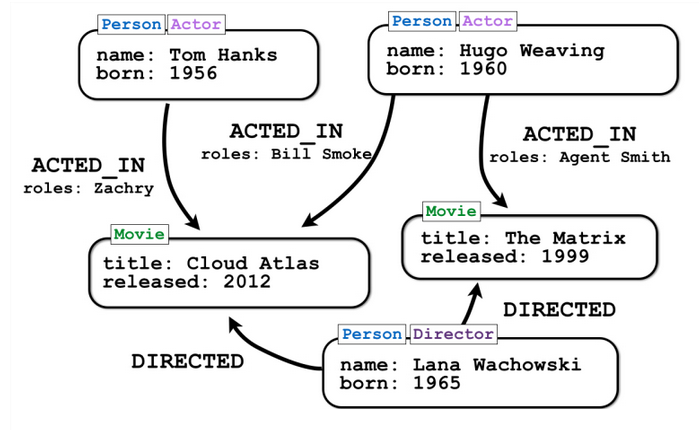
\includegraphics[width=1\textwidth]{images/graphe.png}
			\caption{Exemple de graphe.}
		\end{figure}
	\end{frame}

	\begin{frame}
		\frametitle{Bases de données orientées graphes}

		\begin{itemize}
			\item \textbf{Modélisation :} représentation de l'information de manière très particulière (nœuds et arcs de même importance) ;
			\item \textbf{Opérations :} traitement très particulier de l'information (voir slide précédente) ;
			\item \textbf{Cas d'utilisation :} utilisé principalement pour les réseaux (liens entre des équipements ou des personnes) ;
			\item Base de données rarement utilisée pour du stockage ;
			\item \textbf{Principaux acteurs :} Neo4j, Titan, OrientDB.
		\end{itemize}
	\end{frame}

	\begin{frame}
		\frametitle{Bases de données orientées graphes}

		\begin{figure}[htb]
			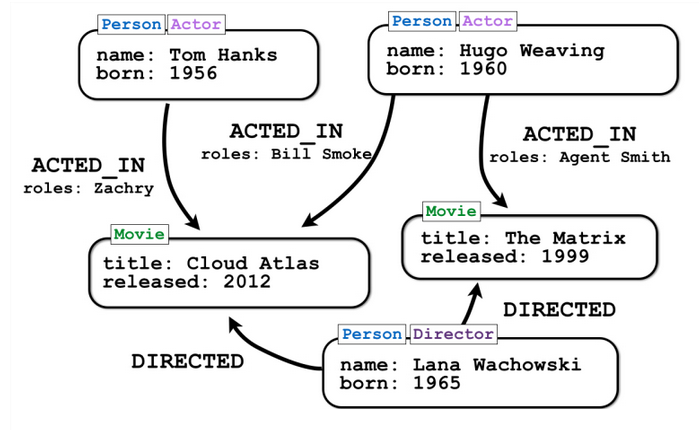
\includegraphics[width=1\textwidth]{images/graphe.png}
			\caption{Exemple de graphe.}
		\end{figure}
	\end{frame}

	\begin{frame}
		\frametitle{Exemple de requête}

		\begin{figure}[htb]
			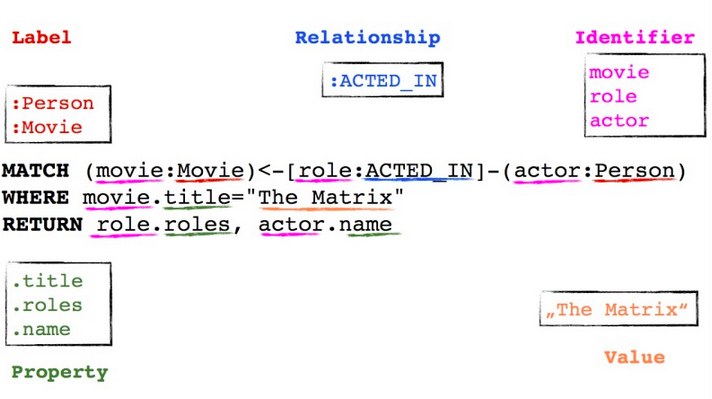
\includegraphics[width=1\textwidth]{images/requeteNeo4j.png}
			\caption{Exemple de requête Cypher pour Neo4j.}
		\end{figure}
	\end{frame}


		\section{Conclusion}

	%% Bonnes pratiques
	\subsection{Bonnes pratiques}
		\begin{frame}
			\frametitle{Les bonnes pratiques du NoSQL}

			\begin{itemize}
				\item Ne pas commencer par du NoSQL ;
				\item Bien connaître ses données ;
				\item Ne pas avoir peur de la redondance ;
				\item Ne pas trop redonder ;
				\item Et surtout, bien quantifier ses besoins.
			\end{itemize}


			\begin{block}{RTFM}
				La majorité des bases de données NoSQL connues sur le marché possèdent une très bonne documentation, souvent faite à destination de personnes venant du monde du relationnel.
			\end{block}
		\end{frame}

		\begin{frame}
			\frametitle{D'autres cas d'usage du NoSQL}
			\begin{alertblock}{Première ligne en prod', mais pas que}
				Le NoSQL ne permet pas uniquement de contenir la charge, de répondre aux problématiques du distribué.
			\end{alertblock}

			\vspace{10px}

			D'autres attraits du NoSQL:
			\begin{itemize}
				\item \textbf{Dénormalisation:} business intelligence, machine learning, data mining (BDD colonnes, documents)\dots
				\item \textbf{Stockage:} entrepôt d’agrégation de données (BDD colonnes, documents)
				\item \textbf{Modélisation:} systèmes de recommandation (BDD graphe)
				\item \dots
			\end{itemize}
		\end{frame}

	%% NoSQL ou relationnel ?
	\subsection{NoSQL ou relationnel ?}
		\begin{frame}
			\frametitle{NoSQL ou relationnel ?}

			\begin{alertblock}{Les deux mon capitaine !}
				Les bases de données NoSQL ont été inventées afin de résoudre des problèmes insolubles par les bases de données relationnelle et non \textbf{pas pour les remplacer}.
			\end{alertblock}

			\vspace{20px}

			\begin{tabular}{|l|l|}
				\hline
				\textbf{NoSQL} & \textbf{Relationnel} \\ \hline\hline
				stockage de masse & stockage fiable \\ \hline
				données diverses & données formatées \\ \hline
				scalabilité horizontale & scalabilité verticale \\ \hline
			\end{tabular}
		\end{frame}

		\begin{frame}
			\frametitle{Choix du type de BD NoSQL}

			\begin{tabular}{|p{0.20\textwidth}|p{0.40\textwidth}|p{0.30\textwidth}|}
				\hline
				& Modélisation & Cas d'utilisation \\\hline
				Clé / valeur
				& Modélisation simple, permettant d'indexer des informations diverses via une clé
				& Mise en cache  \\\hline
				Documents
				& Modélisation souple permettant de stocker des documents au format JSON dans des collections
				& Stockage de masse \\\hline
				Graphes
				& Modélisation optimisée pour les problèmes de graphes
				& Stockage provisoire pour traiter les données \\\hline
			\end{tabular}

			\vspace{10px}

			Non exhaustif: il existe d'autres types de BDD NoSQL !
		\end{frame}


\end{document}